\section{Video Segmentation and Classfication}
\subsection{Video Segmentation}
For video segmentation, we use the software proposed by (cite), which enables fast shot segmentation using global and local visual descriptors. This method can generate segments of shots from one video, which has fairly high accuracy. We did not use scene segmentation, since the scenes can be segmented by classification results - we can combine the continuing shots with the same label into a scene of the label, thus finishing the task fo scene segmentation using shot segmentation.
\subsection{Video Classification Pipeline}
After shots are segmented from a video, we train a classifier to predict the label for one particular shot. For speed and scalability, we extract two feature vectors from the frames and sound of the shot respectively; Then, we train these feature vector separately using popular classfication techniques such as the support vector machine(cite needed); Finally, we combine the weights of the two classifiers by selecting a weight parameter $p$, where $0 < p < 1$. \par
The reason we train two classifiers separately is as follows:
\begin{itemize}
\item The dimensions of the feature vector from frames and sound vary significantly. For popular image classification techniques(cite HOG and SIFT), thousands of features can be extracted from one image, whilst for the audio feature extraction technique MFCC(cite needed), the length of feature vector is 12.
\item In some cases, using only the frame(or the audio) data could lead to false predictions. For example, when a news show is reporting wildlife protection, using only the frame data would likely result in labeling the shot as "nature", but we can ascertain that the shot is "news" based on the voice of the speaker.
\end{itemize}
In both settings, we use the LIBLINEAR library for our SVM classifier, which narrows the classification problem down to feature extraction.
\subsection{Frame Feature Extraction Techniques}
Feature extraction for a particular frame is largely equivalent to image feature extraction. Therefore, popular image feature extraction techniques are used in our methods. In the following subsections, we present three techniques.
\subsubsection{Spatial Pyramid Pooling}(cite)
Let us construct a sequence of grids at level $0 \ldots L$, such that grid at level $l$ has $2^l$ cells along each dimension. For one image, we use average pooling for each grid, and compute one feature. Combining all the features of every grid in every level, and we have $\sum_{l=0}^{L} 4^l$ features extracted from one image. Figure \ref{fig:spp} demonstrates our method.

%\begin{figure}[H]
%\centering
%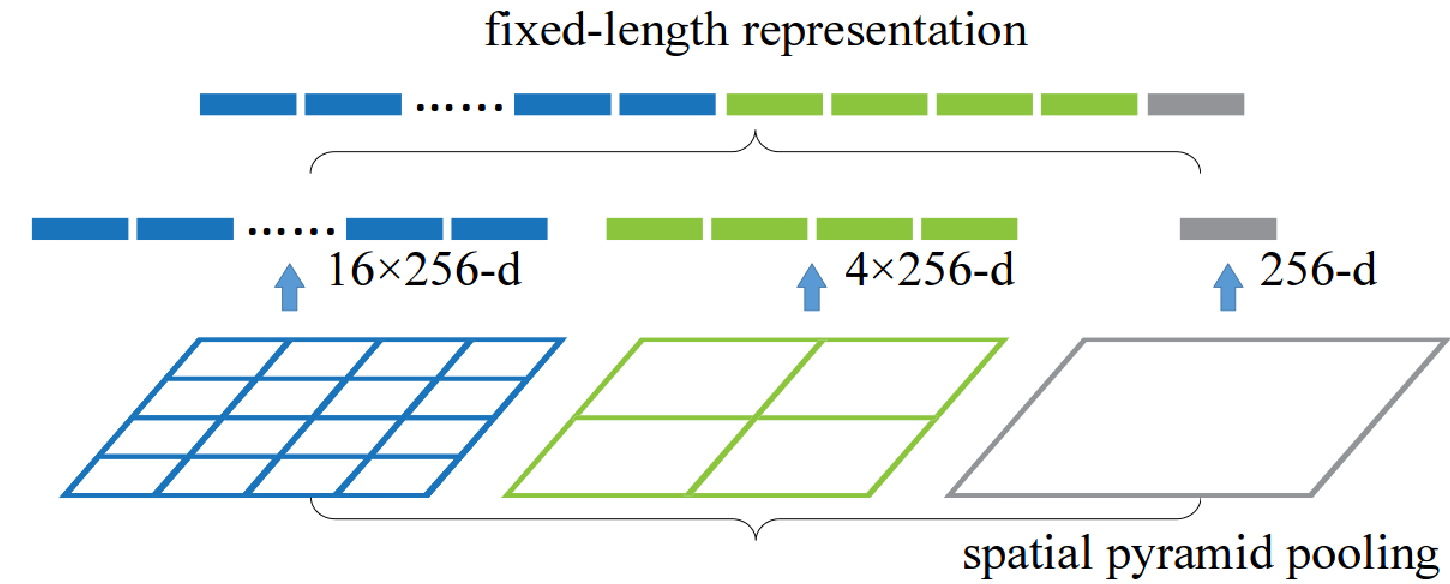
\includegraphics[width=0.8\textwidth]{spp.png}
%\label{fig:spp}
%\caption{Spatial Pyramid Pooling}
%\end{figure}

\subsection{Histogram of Oriented Gradients}
Histogram of Oriented Gradients(HOG) are feature descriptors used in computer vision and image processing for the purpose of object detection. The technique counts occurences of gradient orientation in localized portions of an image. HOG descriptors maintains a few advantages over other methods, since it upholds invariance to geometric and photometric transformations, except for object orientation.\par
HOG descriptors are computed using the following steps:
\begin{description}
\item[Gradient Computation] The first step of HOG computes the gradient values, mostly by using the 1-D centered, point discrete derivative mask in one or both of the horizontal and vertical directions.
\item[Orientation Binning] The second step consists of creating the cell histograms. Each pixel within the cell casts a weighted vote for an orientation-based histogram channel based on values found in the gradient computation.
\item[Descriptor Blocks] The third step involves grouping the cells into larger, spatially connected blocks. The HOG descriptor is then the vector of the components of the locally normalized cell histograms from all of the block regions.
\end{description}
In our setting, we scale each image to size $128 \times 128$ and use non-overlapping blocks of size $32 \times 32$, resulting in a 11340 dimensional feature vector. We further trim the feature vector by $75\%$, using $2835$ features each image for training.

\subsection{Deep Convolutional Activation Feature}
Recent advances in deep learning have enable researchers to apply deep convolutional neural networks(CNN) to large-scale visual recognition tasks. These models perform extremely well in domains with large amounts of training data, outperforming all known methods on a large scale recognition challenge.\par
However, in other tasks with limited training data, deep neural networks tend to dramatically overfit. To deal with this problem, Donahue et al.(cite) explored a semi-supervised, transfer learning method, which uses a supervised pre-trained deep neural network to extract features. One popular feature selection method is to use activation values in one layer of deep neural network. Donahue et al. have empiracally validated that a generic visual feature based on a convolutional network trained on the ImageNet dataset(cite) outperforms a host of conventional visual representations on standard benchmark object recognition tasks.\par
In our setting, we use the famous AlexNet by Krizhevsky et al. (cite), which contains eight layers with weights: the first five are convolutional and the remaining three are fully connected. The output of the last fully-connected layer is fed to a 1000-way softmax which produces a distribution over the 1000 class labels. The structure of the AlexNet is in figure \ref{fig:alexnet}. Please refer to (cite) for more details of the network. \par

%\begin{figure}
%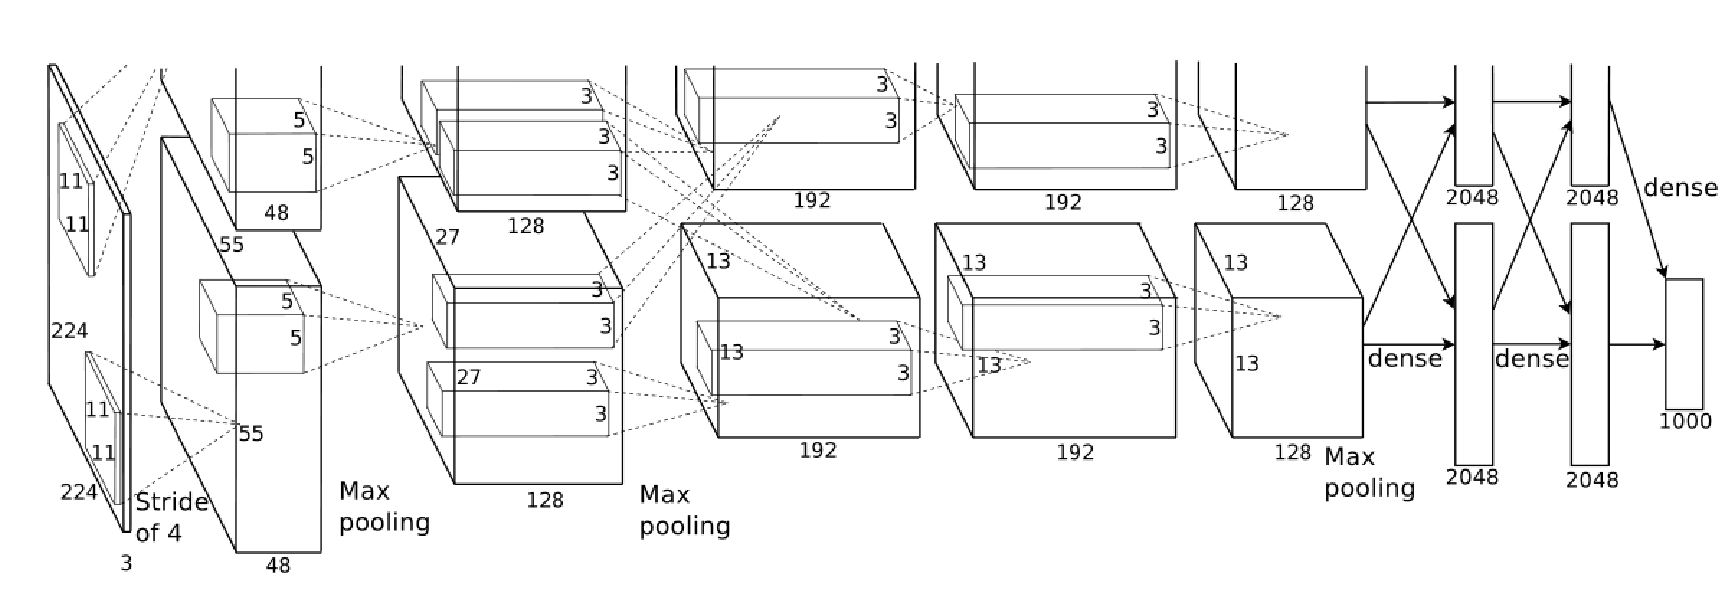
\includegraphics[width=1.0\textwidth]{alexnet.png}
%\label{fig:alexnet}
%\caption{Structure of AlexNet}
%\end{figure}

We use the seventh layer of AlexNet, which has 4096 neuron activations, as our extracted features. We use Caffe(cite), an open source framework for training deep nerual networks on GPUs, and a model trained on ImageNet using Caffe, to extract our features. For each image, we simply do forward propagation, using the image pixel intesities as inputs, and compute the neuron activations of the particular level. Using a GPU, we can speed up the computation by 5 to 10 times.

\subsection{Audio Feature Extraction Techniques}
\subsubsection{Mel-Frequency Cepstrum Coefficients}
In sound processing, the mel-frequency cepstrum is a representation of the short-term power spectrum of a sound, based on a linear cosine transform of a log power spectrum on a non-linear mel scale of frequency. Mel-frequency cepstrum coefficients(MFCCs) are coefficients that collectively make up an MFC, which are derived from a type of cepstral representation of the audio clip. MFCCs are commonly derived as follows:
\begin{enumeration}
\item Take the Fourier transform of a signal
\item Map the powers of the spectrum obtained above onto the mel scale, using triangular overlapping windows.
\item Take the logs of the powers at each of the mel frequencies.
\item Take the discrete cosine transform of the list of mel log powers, as if it were a signal.
\item The MFCCs are the amplitudes of the resulting spectrum.
\end{enumeration}
In our setting, we compute the average MFCCs for each shot, so that each shot generates a 12-dimensional feature vector.
\subsubsection{Linear Prediction Coefficients(LPCs)}
Linear prediction is a mathematical opearation where future values of discrete-time signal are estimated as a linear function of previous samples. The most common representation is 
$$ \hat{x}(n) = \sum_{i=1}^{p} a_i x(n-i)$$
where $\hat{x}(n)$ is the predicted signal value, $x(n-i)$ is the previous observed values, and $a_i$ are the predictor coefficients. The error generated by this estimate is 
$$ e(n) = x(n) - \hat{x}(n)$$
where $x(n)$ is the true signal value. \par
The most common choice in optimization of parameters $a_i$ is the root mean square criterion which is also called the auto-correlation criterion. In this method we minimize the L2 norm, which yields the equation:
$$\sum_{i=1}^{p} a_i R(j-i) = -R(j)$$
for $1 \leq j \leq p$, where $R$ is the auto correlation of signal $x_n$, defined as
$$R(i) = \mathrm{E}[x(n)x(n-i)]$$
and $\mathrm{E}$ is the expected value.\par
In our setting, we compute a 12-dimensional feature vector for the LPCs, which gives us a feature vector of length 24 after combining with MFCCs.


